\documentclass[11pt,dvipsnames]{article}

%\renewcommand{\familydefault}{\sfdefault}

% include some packages
\usepackage{xurl}
\usepackage[left=2cm,right=2cm,top=2cm,bottom=3cm]{geometry}
\usepackage{graphicx}
\usepackage{tikz}
\usetikzlibrary{shapes,backgrounds,calc,arrows,fit,positioning, quotes}

\usepackage{floatrow}
\usepackage{float}
\usepackage{parskip}
\usepackage{microtype}
\usepackage{xcolor}
\usepackage[setpagesize=false,pdftitle={Parallel code generation on the CPU},pdfauthor={Xiu Nuan Lim}]{hyperref}
\usepackage{textcomp}
\usepackage{minted}
\usepackage{relsize}
\usepackage{xspace}
\usepackage{subcaption}
\usepackage{rotating}
\usepackage{longtable}
\usepackage[style=iso]{datetime2}

\newcommand{\specialcell}[2][c]{%
  \begin{tabular}[#1]{@{}c@{}}#2\end{tabular}}
  
 % \newcommand{\helpme}[1]{{\color{red}#1}}
  
\newcommand{\bigcomment}[1]{}

% \usepackage{fontspec}
% \setmainfont{[Monocraft.otf]}
% \setsansfont{[Monocraft.otf]}
% \setmonofont{[Monocraft.otf]}

\newcommand{\icpp}[1]{\mintinline[breakanywhere]{cpp}{#1}}
\newcommand{\mono}[1]{\texttt{#1}}
\newcommand{\Rplus}{\protect\hspace{-.1em}\protect\raisebox{.35ex}{\smaller{\smaller\textbf{+}}}}
\newcommand{\Cpp}{\mbox{C\Rplus\Rplus}\xspace}
\newcommand{\CppXI}{\mbox{C\Rplus\Rplus11}\xspace}
\newcommand{\CppXVII}{\mbox{C\Rplus\Rplus17}\xspace}
\newcommand{\CppXX}{\mbox{C\Rplus\Rplus20}\xspace}

\renewcommand{\arraystretch}{1.28}

\AddToHook{cmd/section/before}{\clearpage}

% https://tex.stackexchange.com/a/847/172801
\hypersetup{
    colorlinks   = true,
    pdfnewwindow = true,
    linkcolor    = black,
    citecolor    = {ProcessBlue!80!black},
    urlcolor     = {blue!80!black}
}
\def\sectionautorefname{Section}
\def\subsectionautorefname{Section}
\def\subsubsectionautorefname{Section}

\frenchspacing
\setlength{\parindent}{0pt}

\counterwithin{table}{section}
\counterwithin{listing}{section}

\begin{document}

\thispagestyle{empty}

\includegraphics{UL_Algemeen internationaal_CMYK}

\vspace{-2cm}\hfill \begin{LARGE}\textbf{Bachelor Computer Science}\end{LARGE} \\

\vspace{3.5cm}
\begin{Large}
\hfill Parallel code generation on the CPU

\vspace{2.5cm}

\hfill Xiu Nuan Lim
\end{Large}

\vspace{6cm}

\begin{large}

Supervisors:\\
Dr. K. F. D. Rietveld


\vspace{2.8cm}
BACHELOR THESIS

\vspace{5mm}
Leiden Institute of Advanced Computer Science (LIACS)\\
\href{https://liacs.leidenuniv.nl}{\underline{\texttt{https://liacs.leidenuniv.nl}}}\hfill dd/mm/yyy
\end{large}

\newpage



\begin{abstract}

\noindent
Compilers are usually single-threaded programs, sequentially translating source code into executable machine code. By taking advantage of modern multi-core CPUs equipped with explicitly parallel SIMD instructions, we adapt previous work performing this task on GPUs to work on conventional CPUs. This results in an implementation of a parallel compiler capable of higher throughput than a traditional, fully sequential approach would yield.

This thesis describes Ptilopsis, an AVX2-based multithreaded CPU implementation of the backend of a parallel compiler, which is capable of transforming an abstract syntax tree into RISC-V code using novel compiler steps described in previous work. Experimental evaluation of these steps using various types of input data shows that Ptilopsis compares favorably to a GPU-based implementation. A number of bottlenecks present on the GPU-based implementation are not present on the CPU, while others remained unaffected.

\end{abstract}

\thispagestyle{empty}
\tableofcontents
\thispagestyle{empty}

\clearpage
\setcounter{page}{1}

\section{Introduction} \label{introduction}
Compilers serve a vital part in software development, as these programs are what allow developers to express their programs in higher-level concepts and not have to worry about how these concepts eventually translate into executable machine code. Despite optimization efforts, compilation still remains a primarily single-threaded process. Because of this, modern build systems often run multiple instances of the compiler in parallel to try and improve the total throughput. Despite this, utilization often is not optimal, and large source files can still take a significant amount of time to compile.

Previous work described Pareas \cite{voetter2021} \cite{huijben2021} \cite{pareas22}, a parallel compiler running on a GPU written in Futhark \cite{futhark}. Due to the SIMT nature of GPU architectures, it is not suitable to simply run each step of the compiler in parallel or to run multiple instances of the compiler. Therefore, the steps a traditional compiler uses to achieve the described transformation were redesigned to be more efficiently parallelized for execution on a highly parallel processor such as a GPU. These efforts resulted in a very high total throughput, especially for large input files.

In this thesis, we investigate the effectiveness of applying these same modified compiler steps using SIMD while running on a multi-core CPU. To do so, we describe Ptilopsis, a compiler backend based on Pareas, which transforms a previously generated abstract syntax tree into binary RISC-V code in a parallel manner. The backend was specifically chosen for investigation because of its reliance on many similar operations, in this case, tree walk operations. For the implementation of Pareas conventional pointer-based tree operations were modified into operations on contiguous data representing the AST as what is effectively a parent point tree, stored in array form, called an inverted tree. For Ptilopsis, these operations were adapted to work on a conventional CPU using AVX2 intrinsics \cite{intrinsics} and multiple CPU threads.

Ptilopsis is available on GitHub at \url{https://github.com/TypeA2/Ptilopsis}.

\subsection{Overview}
In this thesis, we describe the implementation, workings, and effectiveness of the Ptilopsis compiler backend, as well as compare it to that of Pareas.
\autoref{background} will outline the workings of traditional compilers, the usage of Single Instruction, Multiple Data (SIMD) instructions and intrinsics, and considerations when using the \Cpp programming language for the task of implementing a parallel compiler.
\autoref{implementation} describes the individual steps performed by the compiler and how the implementation of Ptilopsis differs from that of Pareas.
In \autoref{experiments} various experiments are performed in order to characterize the implementation's performance with multiple different kinds of input files.
Finally, in \autoref{discussion} the results and implications of these results are discussed and compared to those of Pareas. Additionally, limitations as well as possible future improvements to the backend are identified.

\section{Background} \label{background}
\subsection{Compilers}
In general, a compiler can be said to consist of two phases: analysis and synthesis \cite{compilerbook}. The analysis phase takes the original source code as its input and transforms it into an intermediate representation suitable for the synthesis part to work with. This transformation also includes verifying the code's syntactic and semantic validity and providing feedback to the user if there is an issue with these properties. Afterward, the synthesis phase generates an actual executable program from this intermediate representation and other relevant information gathered by the analysis phase, like a symbol table. The analysis and synthesis parts are often called the front end and back end respectively. A schematic overview of the steps that make up these phases is shown in \autoref{fig:dataflow}. In practice, not all compilers perform all these steps, and often multiple steps are combined into one, removing the need for an intermediate representation. Traditional compilers perform these different stages in sequence using a single CPU thread.

\begin{figure}[!ht]
    \centering
    % https://tex.stackexchange.com/a/146320/172801
    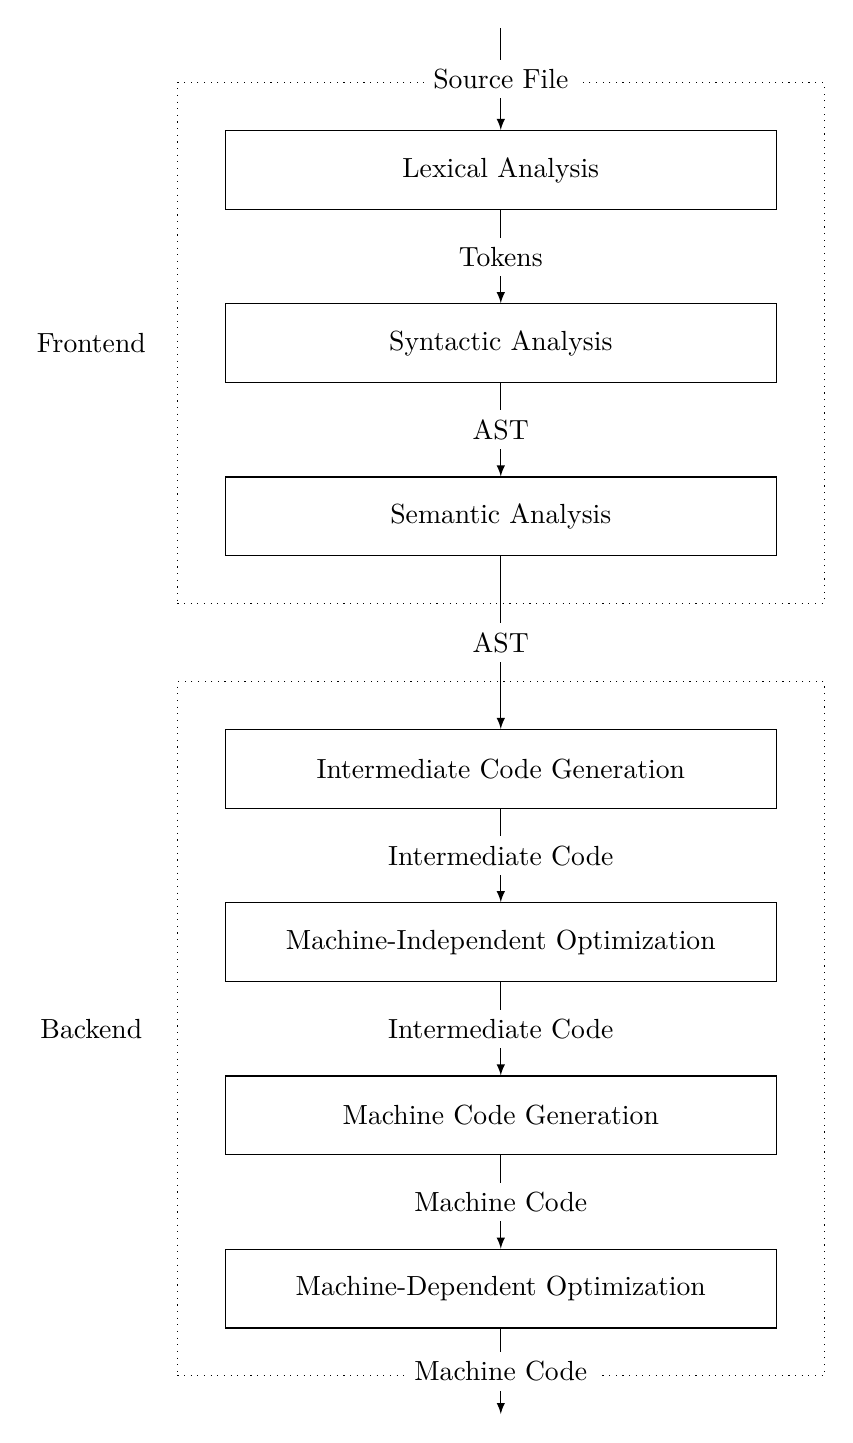
\begin{tikzpicture}[
            node distance = 2.2cm,
            data/.style={
                draw,
                rectangle,
                minimum width = 7cm,
                minimum height = 1cm
            },
            every edge quotes/.style = {fill = white}
        ]
        \node[data] (lex) {Lexical Analysis};
        \node[data, below of=lex] (syntax) {Syntactic Analysis};
        \node[data, below of=syntax] (semantic) {Semantic Analysis};
        \node[data, below of=semantic, below=0.5cm] (intermediate) {Intermediate Code Generation};
        \node[data, below of=intermediate] (indep_opt) {Machine-Independent Optimization};
        \node[data, below of=indep_opt] (gen) {Machine Code Generation};
        \node[data, below of=gen] (dep_opt) {Machine-Dependent Optimization};
        
        \node[draw,dotted,fit = (lex) (syntax) (semantic), inner sep=0.6cm] (frontend) {};
        \node[left=3cm, left of=frontend] (frontend_title) {Frontend};
        \node[draw,dotted,fit = (intermediate) (indep_opt) (gen) (dep_opt), inner sep=0.6cm] (backend) {};
        \node[left=3cm, left of=backend] (backend_title) {Backend};
        
        \draw[-latex] (0,1.8cm) to ["Source File"] (lex);
        \draw[-latex] (lex) to ["Tokens"] (syntax);
        \draw[-latex] (syntax) to ["AST"] (semantic);
        \draw[-latex] (semantic) to ["AST"] (intermediate);
        \draw[-latex] (intermediate) to ["Intermediate Code"] (indep_opt);
        \draw[-latex] (indep_opt) to ["Intermediate Code"] (gen);
        \draw[-latex] (gen) to ["Machine Code"] (dep_opt);
        \draw[-latex] (dep_opt) to ["Machine Code"] (0,-15.8cm);
    \end{tikzpicture}
    \caption{Execution phases of a compiler}
    \label{fig:dataflow}
\end{figure}

\subsection{Parallelism}
CPUs typically operate on two conceptual inputs: a stream, or sequence, of instructions to execute and a stream of data to manipulate in a manner described by the instructions in the instruction stream \cite{flynn}. In order to achieve faster processing parallelism (processing multiple elements) may be applied to the instruction stream, the data stream, or both. Different applications of these methods are discussed below.

\subsubsection{Multithreading}
A conventional CPU core executes based on a single instruction stream and a single data stream. This can be considered a Single Instruction, Single Data (SISD) architecture. In the past decades, systems with only a single core have largely been replaced by systems with multiple cores. These cores generally operate independently on their own instruction and data streams, leading to what we call a Multiple Instruction, Multiple Data (MIMD) architecture.

In addition to this, it has been observed that with both of these architectures, the utilization of the individual components is not optimal in most cases, meaning that components may be idle, waiting for data from other components to be ready, while they could be used to process more data. A solution to this is simultaneous multithreading, a technique that allows a single core to execute multiple instruction and data streams, in order to optimize the utilization of its functional units \cite{smt}. This method exposes a single physical core as two "logical" cores to the system running on it, allowing it to be treated in a manner similar to having multiple cores. While the scaling is not perfect, this method does allow for increased parallelism.

\clearpage

\subsubsection{SIMD}
A different approach is a Single Instruction, Multiple Data (SIMD) architecture. With this architecture, a single instruction from the instruction stream specifies the operations to perform on multiple data input streams or on multiple elements from a single stream. This can be the same operation on each input, or different operations depending on what the specification describes. This approach allows multiple data inputs or elements to be processed in parallel, reducing the sequential nature of performing multiple of the same operation.

A major set of SIMD instructions on x86 and x86\_64 platforms are the Intel Advanced Vector Extensions (AVX) \cite{Lomont11introductionto}, and AVX2 \cite{haswell}, which operate on 128-bit and 256-bit data registers respectively. These data registers can be treated like multiple data types: 32 8-bit integers, 16 16-bit integers, 8 32-bit integers, 4 64-bit integers, 8 32-bit floating point, and 4 64-bit floating point values. By allowing these many data types, these extensions are highly flexible.

\subsection{\texorpdfstring{\Cpp}{C++}}
Using the \Cpp programming language, both of the previously mentioned methods of parallelism can be implemented.

Starting from \CppXI the \Cpp standard library has included mechanism for creating multiple threads (\icpp{std::thread}), as well as synchronization mechanisms such as mutexes (\icpp{std::mutex}), locks \linebreak (\icpp{std::unique_lock}) and atomic data types (\icpp{std::atomic<T>}). \CppXX expands upon this, and in particular, provides a re-usable thread coordination mechanism in \icpp{std::barrier}. Using these functionalities, it is possible to have multiple threads running, have each execute a part of an algorithm, and wait for all other threads to have finished execution as well before continuing.

\CppXVII provides explicitly parallelized versions of common algorithms, such as sorting an array or filtering elements. The GCC compiler uses the Intel oneAPI TBB \cite{oneapi} internally for this functionality, while the \mono{MSVC} compiler uses native APIs provided by the Windows OS.

In addition to using the \Cpp standard library, most major \Cpp compilers provide intrinsics for writing AVX and AVX2-based code\footnote{\textit{intrinsics} are functions that are specially handled by the compiler, in this case mapping the functions to one or more AVX or AVX2 instructions.}. Because of \Cpp's compile-time capabilities, it is possible to write wrapper functions for these intrinsics that result in the same instructions being generated as if it were written by hand. Additionally, operator overloading allows for more streamlined usage of these intrinsics, as it is possible to map long intrinsic names such as \icpp{_mm256_add_epi32(a, b)} to common and easily readable operators (\icpp{a + b} for the previous example).

Compilers are sometimes able to identify common patterns in normally written code and compile these to applicable AVX2 instructions when tasked to, but this behavior is limited and unreliable. Ideally, one would write either conventional \Cpp and have the compiler translate this to SIMD code, or write somewhat conventional code within a provided framework and have the compiler still generate SIMD code, similar to how the Futhark language operates. However, due to the nature of \Cpp's compile-time capabilities, these options can be impractical or of limited use. In practice, this parallelization task is usually performed manually by the programmer, by specialized compilers (such as the Intel oneAPI DP\Cpp/\Cpp Compiler \cite{intelcompiler}) or frameworks, or even especially designed programming languages.

\subsection{General-purpose computing on GPUs}
Another common example of modern parallel processing is the modern GPU. When operating these generally have a single instruction stream, but with thousands of individual cores operating on these same instructions and data in parallel. On a high level, these can thus be classified as SIMD. However, it can be useful to further refine this concept. Modern GPUs follow the concept of the \textit{Array Processor} architecture, meaning a single control unit controls many independent processing elements, each with its own registers and optionally storage \cite{flynn2}. Nowadays this is often called a Single Instruction, Multiple Threads (SIMT) processor.

In addition to being SIMT processors, GPUs are also associative, or \textit{predicated} SIMD processors. This means that every compute unit always "sees" every instruction, but only acts upon them when told to do so. This leads us to a major downside of this architecture, namely that branching is expensive, since both branches need to be fully executed by all cores in the system, instead of every core only executing a single branch based on the data it was assigned. Even so, the massive levels of parallelism achieved by these processors often make up for this downside, as well as programming efforts to keep branching to a minimum being able to further reduce the impact. Due to the inherent heavily branching program flow of traditional compilers, these types of programs pose an additional challenge for parallelization.

\subsection{Related Work}
Intel has created the oneAPI TBB library for parallel programming \cite{oneapi}. This library is based on letting the programmer break down computations into smaller tasks that are automatically and efficiently executed on multi-processor systems. This has been shown to scale well to many-core systems and is used by GCC for the implementation of parallel algorithms in the \Cpp standard library, but still suffers from the previously discussed issue that traditional compilation steps simply do not allow for much parallel processing.

\textit{The Parallel GCC} project attempts to parallelize some of the steps of the GCC compiler and shows modest speedup when doing so. However, the overall structure of the compiler is not specifically adapted to parallel processing, and there is only a limited number of steps that are executed in parallel. Notably, it mostly focuses on optimization within individual functions, which presents the same potential problems as faced by the register allocation step of Pareas and Ptilopsis regarding the type of input data, where the level of parallelism scales with the number of functions, leading to source files with very few functions to mostly compile in a sequential manner.

The Vc library, available at \url{https://github.com/VcDevel/Vc}, allows for explicitly data-parallel programming in \Cpp \cite{vc} \cite{Kretz2015}. By defining new types and overloading their relevant operators, this library achieves AVX-based code generation with a more natural syntax than compiler intrinsics. It allows for easy parallelization of data processing tasks without external code generation or manually writing the intrinsics. However, it is still mostly based on operations on individual data elements, instead of higher-level constructs like a language like Futhark may allow, and as such it doesn't provide significant value or ease of programming over similar abstractions that were purpose-written for Ptilopsis.

In the 1980s and 1990s, there was considerable development of parallel architectures, which in turn led to significant interest in the concept of parallel compilers \cite{SKILLICORN1993337}. Despite this, compilers have remained largely sequential programs. Only recently the inverted tree data structure was proposed to aid parallelization \cite{hsu2019data}, and the Pareas compiler is largely based on work from the 1980s and 1990s and on relatively recent work.

\section{Design and Implementation}  \label{implementation}

This section describes how the Ptilopsis compiler backend operates, what changes were made compared to Pareas, and what challenges were encountered. Whereas Pareas is written in Futhark, a language specifically designed for parallelism, we have chosen to implement Ptilopsis in \Cpp. This brings advantages in the ease of use of explicitly parallel AVX2 intrinsics, as well as the option to apply conventional programming methods to aid in implementing the compiler.

\subsection{Primitives}
Most compiler steps follow a load-calculate-store pattern, where data is initially loaded into AVX2 registers, before being manipulated using common arithmetic operations, and using masks for conditionals, before storing the calculated data in the same place or in newly calculated positions. AVX2 has several operations to help with this.

\subsubsection*{Shifts}
AVX2 contains functionality to bit-shift 32-bit elements by a specified amount in the form of \linebreak \icpp{_mm256_slli_epi32}, using \mono{vpslld}, for left-shifts, and \icpp{_mm256_srli_epi32}, using \mono{vpsrld} for right-shifts. However, there is no functionality to shift all 256 bits in a register as a single unit. The larger shift instructions operate on 2 individual 128-bit lanes (\icpp{_mm256_slli_si256} with \mono{vpslldq} and \icpp{_mm256_srli_si256} with \mono{vpsrldq} for left and right shifts respectively). This stems from AVX2 being an extension of AVX, which operates on 128-bit registers instead of 256-bit registers. This restriction allowed these 256-bit operations to be easily split up into 2 128-bit operations. This functionality however is required to implement an efficient SIMD prefix sum operation \cite{Zhang2020ParallelPS}, and as such must be emulated using other instructions. Using AVX-512 it is easily implemented using the \mono{valignd} instruction, but using only AVX2 it must be implemented in a different manner.

For a left shift, the lower 128 bits of the source are first placed in the upper 128 bits of the result, and the other bits are set to 0. When we are shifting by exactly 128 bits, this is already the correct result. For a shift of less than 128 bits \icpp{_mm256_alignr_epi8} (\mono{vpalignr}) is used. This instruction operates on 2 128-bit lanes again, and concatenates the corresponding lanes of both inputs, before shifting the result and storing the lower 128 bits of each lane. Because we previously already performed what is effectively a single 128-bit shift, these 2 lanes are used to shift the lower and the upper halves separately, resulting in effectively a single-lane shift. For a shift of more than 128 bits, the lower 128 bits are always zero, and the original lower 128 bits are at least in the upper 128 bits, so the previously mentioned \icpp{_mm256_slli_epi32} (\mono{vpslld}) is used to shift both lanes further. Since the lower half is already zero, this remains zero. A right shift effectively uses the same approach but instead starts by placing the upper 128 bits from the source in the lower 128 bits of the result, before using the same instructions and methods to emulate the correct type of shift.

\subsubsection*{Load and Store}
The most basic operations are 256-bit loads and stores, which use \icpp{_mm256_load_si256} and \icpp{_mm256_store_si256}, both of which translate to the \mono{vmovdqa} instruction, to load 8 subsequent 32-bit elements into vector registers or store the contents of such a register to memory. These require 32-byte aligned addresses. There are also unaligned versions called \icpp{_mm256_loadu_si256} and \icpp{_mm256_storeu_si256} using the \mono{vmovdqu} instruction. As the aligned load and store operations may perform better than unaligned loads and stores, even when both operate on aligned data, the latter should only be used when it is known that the data is unaligned.

\subsubsection*{Masked Load and Store}
Further refinement comes in the form of masked loads and stores (\icpp{_mm256_maskload_epi32} and \icpp{_mm256_maskstore_epi32}, both using \mono{vpmaskmovd}). Here, along with an address and optionally the data to store, a mask is also passed. For every 32-bit element in this mask, the operation (load or store) is only performed if the highest bit is set. This way, loading irrelevant data can be avoided, and overwriting data we have not manipulated or do not want to overwrite is also avoided, while still having the benefits of AVX2 operations.

\subsubsection*{Gather and Scatter}
Finally, AVX2 contains gather operations, but no scatter operations. A gather operation takes a base pointer and a vector or array of indices and based on a given element size, loads all elements in the index array from memory. This way, 8 non-adjacent 32-bit integers can be loaded from memory into a single AVX2 register. A scatter operation is effectively the reverse, taking a base pointer, array of indices, and an array of values to store, and using these inputs stores each value at the index specified by its corresponding element in the index array relative to the base pointer. The AVX2 intrinsics using 32-bit elements (\icpp{_mm256_i32gather_epi32} and \icpp{_mm256_mask_i32gather_epi32}) both use the \mono{vpgatherdd} instruction, and the latter takes an optional mask and source argument. The former unconditionally loads all elements, and the latter only loads the element if the corresponding upper bit in the mask is set. If this is not the case, the element is copied from the source argument. This can be used to zero out skipped elements, or assign any other value to them. AVX2 lacks scatter operations entirely (see \autoref{avx512}), and as such this is implemented by extracting the AVX2 registers to 8-element \icpp{std::array} instances, and using a normal \icpp{for}-loop.

\subsection{Compiler}
Ptilopsis uses a thread pooling system. This means that all threads that are to be used are started before the actual compilation stage. Every thread is then kept waiting until there is a multithreaded task to be performed, and after execution of the assigned task it goes back to waiting. This minimizes the performance impact of starting up multiple threads. In addition to this, on GCC platforms, a parallel sort is performed on a dummy array twice in order for TBB to populate its global thread pool. When using MSVC, this step is also performed, but in a less controlled manner as the exact details are specified by the Windows Thread Pool API.

The compiler stages are the same as in Pareas, in particular: preprocessing, instruction counting, instruction generation, optimization, register allocation, jump fixing, and postprocessing. Implementation and design choices are the same as described for Pareas in \cite{huijben2021}, and any relevant additions have been detailed below. 

\subsubsection*{AST representation}
The compiler receives an AST in post-order format, which was specifically chosen for Pareas for parallel processing. This means that when nodes are processed left to right they are actually processed from the bottom of the syntax tree upwards. Instead of using nodes based on instances of a \icpp{struct} or \icpp{class} interconnected using pointers to various instances representing AST nodes, like in traditional compilers, all node fields are stored separately in arrays of either signed or unsigned 32-bit integers (\icpp{int32_t} and \icpp{uint32_t}). These arrays are specially aligned on 32-byte boundaries, which is required for processing them with AVX2 instructions. This data type is chosen such that all required types within the language we are compiling can still be represented (namely 32-bit integers and 32-bit floating point numbers), but without compromising on parallelism, as 32-bit elements allow us to process 8 elements with a single AVX2 instruction, compared to just 4 with 64-bit elements. This, along with the RISC-V code being limited to the 32-bit subset, means the compiler almost entirely operates with 32-bit operands. Every node contains 6 logical fields: node type, node data type, index of the parent node, depth of the current node, child index (the number of nodes with the same parent preceding this node), and a generic node data field. Details can be found in \autoref{ast}.

When the AST is generated, the node and data types used correspond to those used in the Pareas compiler. These are first translated to Ptilopsis-specific types, which are designed with specific bit patterns that can make later operations using AVX2 instructions easier (see \autoref{ast}), without changing the semantic meaning. In a full implementation, the frontend would output the correct types, so this step is only needed so we can reuse the existing parser, and because of this the translation step is not benchmarked.

\subsubsection*{Register types}
When initially generating registers, the compiler differentiates between \textit{virtual} registers and \textit{physical} registers. Physical registers are stored as integers 0 through 63, values 0 through 31 representing \mono{x0} through \mono{x31}, and values 32 through 63 representing \mono{f0} through \mono{f31}. Virtual registers are stored as integers 64 and higher. As described in \cite{huijben2021}, the exact virtual register used is based on the instruction address.

\subsubsection*{Execution methods}
All compiler steps are processed with either \textit{Singlethreaded AVX2}, \textit{Multithreaded AVX2}, \textit{Singlethreaded Scalar} or \textit{Multithreaded Scalar} code. Due to the limitations of the AVX2 extensions, it is not always possible to implement every part of the code with AVX2 instructions. Most notably, a \textit{scatter} function is missing from AVX2, so this step is always executed in a scalar manner. Similarly, it is not always worthwhile or even possible to implement an algorithm in a multithreaded manner, as setting up the execution does come with an overhead, and potential data dependencies increase this.

\subsubsection{Preprocessing} \label{preprocessing}
Preprocessing prepares the AST for the later stages, allowing for better parallelization and less branching. This stage is performed using multithreaded AVX2 since every node is processed completely independently of all other nodes.

\subsubsection*{Function argument preprocessing}
According to the RISC-V calling convention, integer arguments may be passed in registers \mono{a0} through \mono{a7} or on the stack, and floating point arguments may be passed in registers \mono{fa0} through \mono{fa7}, in integer registers \mono{a0} through \mono{a7}, or on the stack. Based on any function argument node's child index and node data, we can calculate the number of preceding integer and floating point arguments, and thus how the current node should be passed. Function declaration and function call arguments are isolated by making use of the bit pattern properties of the node type as described in \autoref{ast}. Using this mask, for every node that is a floating point argument in an integer register, the lowest bit is set using a bitmask operation. Additionally for every node, if it is either an integer or a floating point argument on the stack, the second bit is set. Finally, the node data field is modified to reflect the new node type. For any arguments in their corresponding natively-typed registers, it is simply the index of the argument register it is stored in. For floating point arguments in an integer register, it is updated to the index of the integer register it is contained in. Finally, if it is an argument on the stack, the node data field is set to the index on the stack, which can be multiplied by 4 in later stages to obtain the byte-based offset. 

\subsubsection*{Function call argument list}
To further simplify later processing we set the node data of function call argument lists to the total number of stack-based arguments. Since the tree is stored in post-order, we can look at the node immediately preceding the function call argument list to get the final argument. If this is a stack argument, its node data is its index on the stack, so adding 1 results in the total number of stack arguments. If this is not the case, however, the number of stack arguments is calculated based on the total number of arguments for each type. Masked store operations are used to update only the argument list nodes' data.

\subsubsection*{Comparison node preprocessing}
All comparison operator nodes have been designed in a similar fashion to function argument nodes. By applying a bitwise AND followed by an equals comparison using the basic equals expression type, we create a mask for all nodes that have a comparison operator of any type as a parent node. Originally these operators return integers for type checking purposes, but for processing into machine code it is more practical for these to return the types they are comparing. Since this means only updating the parent's type when one or more of its children is a floating point node of any kind, we also create a mask for this. For all resulting nodes, we scatter the floating point data type to the data types of the parent nodes.

\subsubsection{Instruction Counting}
The instruction counting stage calculates how many instructions each node generates and where these will be placed in the final executable code. Additionally, a table of all functions is generated, which stores the start index, size, and end index for each function. By pre-calculating the position and size of each instruction, it is possible to perform the compilation of each node independently, since the position in the resulting instruction buffer will already be known.

\subsubsection*{Initial counting}
The first step of the instruction counting stage calculates the base position and size of each node. These will later be adjusted depending on the context of the nodes. This initial calculation is based on information relating to the node and a lookup table, allowing it to be performed using multithreaded AVX2 since all nodes are independent of each other. First, the node type and data type are used to obtain a base number which will be used to further calculate node size. Next, an adjustment value is calculated. Using the masking methods described in \autoref{preprocessing}, every function call argument list node's size is incremented by 1, plus 1 per argument node it has as children. These instructions are used for storing the arguments in the correct locations according to the calling convention. Again using a similar masking method, all conditional nodes (\icpp{if}-statement, \icpp{if}/\icpp{else}-statement and \icpp{while}-statement) are isolated. On all 3 of these nodes, if the lowest bit is 0, the first child is the relevant conditional, and if the lowest bit is 1 the second child is the conditional node. Then, if a node is the conditional node of any of these conditional nodes, the size is incremented by 1. Finally, the size of the second child of an \icpp{if}/\icpp{else}-statement, so the node containing the \icpp{else}-branch, is also incremented to accommodate the unconditional jump over this block when it's not executed.

\subsubsection*{Offset calculation and correction}
Based on the previously calculated node sizes, using a singlethreaded AVX2 prefix sum \cite{Zhang2020ParallelPS}, the preliminary offset for each node is calculated. Next, for every node that is the conditional node for a branching statement, the position of the node is set to the \textit{end} of its allocated space. Profiling has shown that on small inputs (~5 KiB), this step accounts for 2.1\% of the total execution time of the instruction counting step, which grows to 8.0\% on the largest input (50 MiB) when the entire program uses only 1 thread. When using 32 threads in total, the related overhead causes the fraction of time spent on this step to shrink to 0.56\% on the smallest input. When operating on the largest (50 MiB) input using 32 threads, this singlethreaded component represents between 21\% and 25\% of the total execution time for the instruction counting step. Since instruction counting represents a very small segment of the total execution time, it was decided to implement this in a singlethreaded manner. This pattern of marginal gains has shown to also hold in other places where a prefix sum is used, so these are implemented in a singlethreaded manner for the same reason. In addition to calculating the preliminary offsets, the positions of all function call arguments are set relative to their parent node (which will always be a function call argument list). This adjustment step is executed using multithreaded AVX2.

\subsubsection*{Function table generation}
Finally, using singlethreaded AVX2, a table containing all needed information for all declared functions is generated. Using a simple equals comparison and store operation, the node index of every function declaration is stored. Using these indices, the previously calculated locations for these declarations are loaded, and the offset of every function is set to 6 plus this value (the 6 instructions are used for managing the function's stack frame). After this, function sizes are calculated by looking at the offset of the next function using unaligned reads, and finally, the function end indices are calculated using the function offsets and function sizes. The level of parallelism that is able to be achieved by these steps is limited to the number of functions present in the input. As is shown in \autoref{shape}, regardless of the number of functions in the input, the instruction counting step represents a very small part of the total execution time, so there a. In addition to this, these operations are largely loads and stores, so further investigation should be done to determine whether memory bandwidth represents a significant bottleneck.

\subsubsection{Instruction Generation}
The instruction generation step is responsible for calculating what opcodes are used to represent each node. The node types have been chosen to work well with this step. Instruction generation works in parallel on every level of the AST. This is because information about child nodes may be needed to properly compile some nodes. To achieve this scheduling, the compiler first generates an array containing the index for every node. This is then sorted using multithreaded scalar code based on the depth field of the corresponding node. Next, the start indices for all levels are isolated, again with multithreaded scalar code. This is done by comparing the depth of every node in the sorted list to the depth of the previous node. If this value has changed, this means the current depth level has changed, and the value is stored. Following this, starting from the bottom of the AST and working upwards, every level is processed individually using multithreaded AVX2. Since every node is designed to generate at most 4 instructions, it is possible to process 2 nodes at a time with AVX2.

Using the node type, data type, and an index between 0 and 3 for each node, a gather operation is used to, for each of the 4 instructions in every node, obtain whether there is actually an instruction at the specified location. It is important here that no work is done on the second instruction in the AVX2 vector if it does not exist. Unlike Pareas, where the nodes are generated and the data to propagate to higher levels is stored and scattered to the relevant locations afterward, Ptilopsis stores these immediately after the generation step for each of the 1 or 2 nodes. This is not a problem for the algorithm, as it does not rely on values being unwritten or zero initially. Using the same previously described masking and gather operations, the opcode, jump targets, and virtual registers are calculated, and at the end, any data that needs to be propagated to the parent node is scattered using a normal loop. This is repeated for every node in every level, working upwards. Pareas generates all these instructions and then uses a scatter operation to store them at the correct location, just like the propagation data. Ptilopsis instead stores the instructions directly, as this part of the algorithm also does not rely on unwritten data being read as zero, this still is valid, and prevents unnecessary allocations. 

\subsubsection{Optimization}
The main implemented optimization is dead expression elimination, but other optimizations could be adapted to efficiently be applied here, as long as they do not rely on the physical registers. Initially, using multithreaded AVX2 code, all registers that are read from (so registers that appear as \mono{rs1} or \mono{rs2} in any instruction) are marked as used. Following this, a set of optimizations is applied in a loop until there are no optimizations applicable anymore in the resulting code.

For every iteration, two steps are executed using multithreaded AVX2. First, for every instruction, if its destination register is a virtual register and it is not used, both source registers (if present) are marked as unused as well. After this, for every instruction, if it is a store instruction, the source register is marked as used, since this is required for stores to actually work. These two steps are repeated until no registers are marked as unused or used in a single iteration.

Finally, in order to create a mask for all instructions on whether they are enabled after the optimization step, a multithreaded AVX2 operation is used to create a mask which, for all instructions, indicates whether it should be considered in later steps of the compilation process. A mask is used since resizing the instruction arrays is an expensive operation, and masking out unused instructions is relatively cheap. All instructions that have a physical destination register (which may be used for stack frame setup or other related matters) or are marked as having any register in-use are marked as used.

\subsubsection{Register Allocation}
Register allocation translates all present virtual registers to physical registers. To do this, it must keep track of all registers currently in use. This inherently requires a sequential approach, so to still be able to make use of parallelism, instead of processing each instruction in parallel, every function is processed in parallel. Using multithreaded AVX2, all functions are divided among all threads. Every thread processes at most 8 functions at a time since our base unit is still a 32-bit integer. The amount of iterations is decided by the number of instructions in the largest function.

Within every function, the occupation of every register is kept track of in a bitmask. Since there are 64 possible registers, we use 64-bit integers for this, every bit representing one of our physical registers. Since we process 8 functions at a time, this means we require 2 256-bit AVX2 vectors to keep track of this. For this, we duplicate the relevant arrays, with a \mono{*\_lo} and a \mono{*\_hi} variant. Aside from this usage mask, every function also has a preservation mask which indicates what registers have been used within the function. This is necessary when a function is called, as some of the physical registers must be saved by the caller before a function. When the compiler encounters a function call instruction, all physical registers that must be preserved are swapped to the stack, and the registers they reside in are considered free for re-use.

The registers that need to be allocated always contain a specific, often name-carrying symbol. After instruction generation, these are represented by virtual registers. Since the virtual registers are read-once, this means a symbol may be split up into multiple sub-symbols, but the end result is the same. Aside from the previously mentioned masks, the compiler also keeps track of a mapping that maps the physical registers to the symbols currently residing in it. The symbols are represented by the virtual register they originate from and a field that indicates whether it is currently swapped out to the stack. Additionally, the compiler keeps track of a mapping that maps virtual registers (or symbols) to the physical register they currently reside in. In order to preserve consistency, a copy of this mapping must be made for every iteration, to be able to look back at the unmodified. Normally, the processing of every function would have to wait for a single thread to copy over 64 32-bit elements for every function. Since we divide the load across multiple threads, every thread only has to copy over 64 32-bit elements for every function that was assigned to it. This step was measured to form a bottleneck when running on a single thread, so this is an important part of parallelization (for more details see \autoref{experiments}). Pareas generates all register allocation results before performing a scatter operation, but Ptilopsis writes the results after each iteration. As with the instruction generation, because this only relies on already-generated data, the result is the same, but a lot of allocation and memory accesses have been avoided.

After the allocation step itself, using multithreaded AVX2, new instruction sizes are calculated in parallel for each instruction. For each instruction, if it still has a virtual source or destination register, its size is incremented by 1 to make space for the load instruction required to load in the swapped-out value. Next, also using multithreaded AVX2, the start and end instructions for each function are expanded to make space for the instructions required to store and load the preserved registers used by that specific function. A singlethreaded AVX2 prefix sum is used to calculate the new instruction offset. Finally, a multithreaded AVX2-based loop is used to scatter all instructions to their new locations. Where needed, symbols are loaded into temporary registers (\mono{t0} for integer and \mono{ft5} for floating point symbols) and stored on the stack. The resulting instructions are inserted directly into the new arrays storing them. After executing the steps as described in \hyperref[functab]{Function table fixing} to make sure the function positions have been adjusted, the instructions for storing and loading preserved registers are inserted. This partially works with multithreaded AVX2, but since there is no AVX2-based \mono{popcount}, parts have been done in scalar code. The full instruction words with opcode, source, and destination are generated and inserted in the space at the start and end of each function that was previously allocated for this purpose.

\subsubsection*{Function table fixing} \label{functab}
A step that is executed more than once is function table fixing. This step is performed whenever instructions are inserted or removed, so an instruction offset table is passed to this step, which indicates the new index of every instruction. This table is processed by a multithreaded AVX2 loop which adjusts the function start indices, function sizes, and function end indices to their new locations.

\subsubsection{Jump fixing}
Jump fixing inserts needed instruction in order to properly load jumped-to addresses, since these require multiple instructions to load in RISC-V. First, using a multithreaded AVX2 operation, a bitmask is used to isolate all unconditional jump instructions, and their instruction size is set to 2. Using a singlethreaded AVX2 prefix sum, a new position for every instruction is calculated again.

Using multithreaded AVX2, the necessary instructions are inserted to load the full addresses. For direct jump instructions (unconditional jumps), an \mono{auipc} instruction is inserted, which along with the original instruction results in a normal \mono{auipc}-jump pair. For branching instructions (conditional jumps), there is no facility to use a pre-calculated address, but the immediate value must be calculated as a relative offset to the instruction. The relevant bits are directly inserted in the correct position in the instruction word. All these bitwise operations are independent of each other, and part of the instructions AVX2 supplies, so they can be efficiently executed in parallel.

Finally, the steps described in \hyperref[functab]{Function table fixing} are executed again.

\subsubsection{Postprocessing}
Postprocessing merges the generated instruction words together with the source and destination registers. RISC-V always places \mono{rd}, \mono{rs1} and \mono{rs2} at the same position in the instruction word, so these are just shifted into position and combined with a bitwise OR, before being stored in the instruction buffer. This happens with multithreaded AVX2.

\subsection{Scalar version}
In order to help with implementing the optimized parallel version, a version of the Pareas/Ptilopsis backend was implemented that tries to match the original Pareas implementation as closely as possible, using only singlethreaded scalar code. As such, it is highly inefficient when it comes to factors like the number of allocations and memory accesses, but it serves as a baseline to demonstrate the effectiveness and scalability of the (multithreaded) AVX2 implementation.

\subsection{Challenges}
As noted previously, a major functionality missing from AVX2 is the scatter primitive. Although the scalar implementation can easily replace this, it has not been benchmarked whether this significantly impacts performance. 

A major challenge was dealing with conditionals and AVX2. Generally, masks are used to only modify elements that we intend to modify, but this does suffer from the same problem that GPUs exhibit, where some units are effectively idle because their specific assigned element is skipped by the conditional. An attempt has been made to minimize this by not executing certain branches entirely when no element of the mask is set. Despite this, whenever a branch occurs in the AVX2 code, there is a high likelihood that some elements are excluded, leading to an effective decrease in parallelization.

While multithreading does increase core utilization, it does bring overhead. Setting up each thread's task can be costly, and locking efficiently is not trivial. As such, not every step possible has been made multithreaded, as some steps did not pose a significant bottleneck in the entire process, even at the largest tested input size of 50MB, and the performance gained by the parallelization of these steps would not make up for the additional overhead introduced by distributing the work over multiple threads.

\section{Experiments} \label{experiments}

In order to evaluate the various AVX2 and multithread components of Ptilopsis, various experiments were run using the same files that were used to evaluate Pareas, and the results are compared. These input files are available through the Pareas repository at \url{https://github.com/Snektron/pareas}, and detailed information regarding the exact specifications of these files can be found in \cite{huijben2021}. These files contain generated source code, which is first parsed to a pointer-based AST using conventional methods in \Cpp, before being passed to the Ptilopsis backend in the previously described inverted tree format.

The first set of test files (subfolder \mono{basic}) tests the impact of increasing the AST size on the execution time. The second set of test files (subfolder \mono{funclen}) tests the impact of increased function sizes with roughly similar total AST sizes. The third and final set of test files (subfolder \mono{shape}) tests the impact of the total height of the AST with a roughly constant total AST size.

For each experiment, statistics have been collected across 15 runs of the program. Only the execution time of each individual step was taken into account in order to negate any effects the testing instrumentation might have on the final results. This means the initial input parsing and external data structure setup time are not measured. However, the execution time for setting up or copying all data structures and buffers relevant to the compilation itself is taken into account.

Every input file was tested with the following number of threads: 1, 2, 4, 8, 16, 32, 64, 96, 128, 160, 192, and 224 threads. In addition to this, for every combination of thread count and input file, 4 configurations have been tested, named \mono{m0}, \mono{bm0}, \mono{m1}, and \mono{bm1}, with the following command line flags added, the function of which is explained in \autoref{setup}:
\begin{itemize}
    \item Configuration \mono{m0}: \mono{-m 0}
    \item Configuration \mono{bm0}: \mono{-b -m 0}
    \item Configuration \mono{m1}: \mono{-m 1}
    \item Configuration \mono{bm1}: \mono{-b -m 1}
\end{itemize}

All experiments were performed on the same machine, the specifications of which can be found below in \autoref{tab:test_specs}. The compiler used was \mono{g++ (GCC) 12.2.0}.

\begin{table}[ht]
    \centering
    \begin{tabular}{|l|l|}
        \hline
        \textbf{CPU Type} & AMD EPYC 7702 \\
        \hline
        \textbf{CPU Count} & 2 \\
        \hline
        \textbf{Total CPU Cores} & 128 \\
        \hline
        \textbf{Total CPU Threads} & 256 \\
        \hline
        \textbf{RAM Amount} & 512 GB \\
        \hline
    \end{tabular}
    \caption{Hardware specifications of the machine used for the experiments}
    \label{tab:test_specs}
\end{table}

Complete details on reproducing the experiments can be found in \autoref{setup}. All results are listed in \autoref{results}

\subsection*{Note on threading}
Only binaries of Ptilopsis that were built using the GCC toolchain respect the specified thread count, since some parallelism is implemented using the parallel variants of \Cpp STL algorithms like \icpp{std::sort}. These algorithms do not expose an API for limiting the number of threads used. When built using GCC, the compiler uses a backend based on the Intel oneAPI TBB \cite{oneapi}, which can easily be manipulated into limiting the number of total threads. Since no such API exists when compiled using MSVC, this will always use the automatic thread count decided by the Windows Thread Pool API \cite{win32threadpool}.

\subsection{File Size} \label{filesize}
This experiment contains 7 input files, that yield ASTs which all have the same height but an increasing number of nodes and functions. Starting from 1, the total sizes of these input files are roughly 5 KiB, 10 KiB, 100 KiB, 500 KiB, 1 MiB, 10 MiB, and 50 MiB. These test files are structured to be relatively similar to usual real source files, with multiple functions of limited size, and somewhat deep nesting of expressions, leading to a limited, but not a low, total height for the resulting AST.

\autoref{fig:basic_limit} shows the results for a small and a medium-sized test file. Because of the significantly worse performance at high thread counts, the full results for configurations \mono{c} and \mono{d} are not shown here, but these can be seen in \autoref{results}.

From these graphs, we can conclude that at small input file sizes, the overhead for synchronizing multiple threads becomes a major bottleneck. We see some improvements with the 500 KiB input file when using a small number of threads instead of just 1, but in both cases, the performance starts to significantly degrade when using 64 or more threads.

\autoref{fig:basic_limit} also shows the results for the largest 50 MiB source file. From this, we can conclude that on very large inputs there are significant benefits to multithreading, but with diminishing returns. When going from 1 to 2 threads, the total execution time is reduced by around 50\%, but when using 32 threads it is still around $\frac{1}{10}$ of the original execution time. When using more than 32 threads on configurations \mono{c} and \mono{d}, the total execution time starts to increase significantly, likely due to heavy contention on all available cores. On configurations \mono{a} and \mono{b} there is a slight increase in execution time, but not as significant as with the 2 previously mentioned configurations.

In addition to the overall runtime, we can see that, on large input files, parallelization of the register allocation step yields large improvements, while the optimization stage improves moderately and the instruction generation step quite poorly.

It is notable that when using 32 or more threads on small input files, the total execution time starts increasing. This is possibly caused by our testing system being equipped with 2 physical CPUs, leading to performance regression when a task is not running solely on a single physical CPU due to memory access latency.

\begin{figure}[!ht]
    \centering
    \subcaptionbox{5 KiB}{\includegraphics[width=0.49\textwidth]{figures/basic/1_limit_y.pdf}}
    \subcaptionbox{500 KiB}{\includegraphics[width=0.49\textwidth]{figures/basic/4_limit_y.pdf}}
    \subcaptionbox{50 MiB}{\includegraphics[width=0.49\textwidth]{figures/basic/7.pdf}}
    \includegraphics[width=0.49\textwidth]{figures/legend.pdf}
    \caption{Partial data showing the execution time of 3 input files with different total sizes}
    \label{fig:basic_limit}
\end{figure}

\subsection{Function Size}
The second set of experiment files contains 8 input files with roughly the same total size, but a decreasing number of functions. This means that each individual function on average gets longer. This type of input specifically targets the register allocation step, as this is performed sequentially within each function, and only parallelized by the total number of functions.

\autoref{fig:funclen_limit} shows the average execution time for an input file with a very large number of functions, one with a moderate number, and one with a small number of functions. We can see that a smaller number of functions results in a lower execution time, with the fraction represented by the register allocation step shrinking significantly as well. A performance regression when using 32 or more threads is seen just like in \autoref{filesize}, and especially configurations \mono{c} and \mono{d} perform poorly in this situation.

\begin{figure}[!ht]
    \centering
    \subcaptionbox{25118 functions}{\includegraphics[width=0.49\textwidth]{figures/funclen/1_limit_y.pdf}}
    \subcaptionbox{2513 functions}{\includegraphics[width=0.49\textwidth]{figures/funclen/4_limit_y.pdf}}
    \subcaptionbox{100 functions}{\includegraphics[width=0.49\textwidth]{figures/funclen/8_limit_y.pdf}}
    \includegraphics[width=0.49\textwidth]{figures/legend.pdf}
    \caption{Partial data showing the execution time of 3 input files with a differing total number of functions}
    \label{fig:funclen_limit}
\end{figure}

Unlike in \autoref{filesize}, the difference multithreading makes is small, with the biggest improvement visible when a very high number of functions are compiled. When the number of total functions shrinks, the benefit provided by multithreading is reduced. Despite this, we can see that multithreading is most effective in the register allocation step when a high number of functions are present. The instruction generation step sees moderate performance improvement with more threads but seems to be mostly unaffected by the total number of functions present. These results are expected, since instruction generation schedules all instructions based on their level in the AST, regardless of what function they belong to. This is not the case for register allocation, and as such, this step is more affected by a change in the total number of functions.

\subsection{Shape} \label{shape}
The final set of experiment files contains 6 files with corresponding maximum AST depths of 9, 19, 34, 36, 42, and 49. Since function nodes are always located at the second level of the AST, a deeper AST leads to significantly larger functions. \autoref{fig:shape_limit} shows the results for a relatively shallow AST, a moderately deep AST, and a very deep AST. Based on these results we can conclude that, while the instruction generation step is not significantly affected by the depth of the AST, the register allocation step is the main contributor to a high execution time with a very deep AST as input. Since the parallelism of this step is bound by the number of functions, and deeper ASTs necessarily mean larger functions when the total number of functions remains roughly equal, this result is expected as there is less parallelism achievable in large functions.

Based on the results it is also clear that multithreading significantly speeds up this step relative to a single-threaded approach, but the total execution still takes very long on average with very deep ASTs, despite the test files themselves being of similar size.

\begin{figure}[!ht]
    \centering
    \subcaptionbox{9-deep AST}{\includegraphics[width=0.49\textwidth]{figures/shape/1_limit_y.pdf}}
    \subcaptionbox{19-deep AST}{\includegraphics[width=0.49\textwidth]{figures/shape/2.pdf}}
    \subcaptionbox{49-deep AST}{\includegraphics[width=0.49\textwidth]{figures/shape/6.pdf}}
    \includegraphics[width=0.49\textwidth]{figures/legend.pdf}
    \caption{Partial data showing the execution time of 3 input files with varying AST depths}
    \label{fig:shape_limit}
\end{figure}

\subsection{Comparison to Pareas} \label{discussion}

Because of the similarity between Pareas and Ptilopsis, it is possible to use the same files to benchmark them and compare the results to the original results obtained in \cite{huijben2021}.

Pareas was run on an NVIDIA RTX 3090, with 10496 cores and 24GiB of memory, with a bandwidth of 936.2GB/s. Ptilopsis was run on a dual Epyc 7702 system, featuring 64 cores and 128 threads along with 204.8GB/s of memory bandwidth per socket, configured as 2 NUMA nodes. However, it usually performed best when running using 16 or 32 threads, with significant performance regressions when using 64 or more threads. Since the Linux scheduler is NUMA-aware \cite{kernelnuma}, it will attempt to schedule our threads on the same node. At 64 threads, we exceed the number of physical cores per node, so there is a high likelihood that a thread may be scheduled on a physical core of a different node, and this is reflected in our result. Further investigation could be done into the effects of pinning the threads on a single node.

Overall, as was discussed in previous sections, the CPU is better suited for some parts of the compilation process. Specifically, register allocation benefits from the MIMD nature of a multi-core CPU, since branching is not as expensive. Conversely, a SIMT system like a GPU is better suited to processing many individual elements, which is what most other steps of the compilation process consist of. The previously tested workloads are discussed in detail below.

\subsubsection*{File size}

\autoref{fig:scaling_basic} shows the total execution time for different input sizes for Ptilopsis, showing both the AVX2 implementation, and the scalar implementation, compared to that of Pareas. This shows superlinear scaling based on input size for the scalar implementation, as well as roughly linear scaling for the AVX2 implementation and sublinear scaling for Pareas. At low input file sizes, the usage of 32 threads hurts performance. This is expected and was previously discussed in \autoref{filesize}. This effect decreases as the filesize increases, and once the filesize reaches 100 KiB the scaling shows the same characteristics as when using only 1 thread. This is in contrast to Pareas, which performs significantly worse at low filesize, but scales in a sublinear fashion. It is notable that, except for an outlier result at an input size of 1 MiB, the scaling of Pareas across the full range of input files looks similar to that of Ptilopsis when using multiple threads on the smallest four input files. However, there is not enough data on the performance of Pareas on even larger filesizes to confirm this.

\begin{figure}[ht]
    \centering
    \includegraphics[scale=0.8]{figures/basic_scalar.pdf}
    \caption{Comparison of scaling on input size for singlethreaded scalar, singlethreaded AVX2, and multithreaded AVX2 implementations, as well as Pareas}
    \label{fig:scaling_basic}
\end{figure}

Because of the poor parallelization, register allocation on Pareas takes a disproportionate amount of time compared to other stages. At larger input sizes, register allocation is still a major part of the total execution time of Ptilopsis, but it is not nearly as much as in Pareas. This step likely benefits heavily from the independent nature of multiple CPU cores, allowing for a lower performance penalty when branching depending on different parts of the input data, instead of every core having to execute every instruction, regardless of whether that core's assigned data actually uses the result of the branch currently being executed.

\subsubsection*{Function Length} \label{compare_funclen}

\autoref{fig:scaling_funclen} shows the total execution time for a different number of functions with a similar total size for Ptilopsis, again showing the AVX2 and the scalar implementation, compared to that of Pareas. With decreasing function length, and thus increasing total function count, all of the implementations in Ptilopsis initially show a slight execution time decrease, before this starts increasing again. Pareas on the other hand exhibit a significant decrease in total execution time as the number of functions increases, with a slight increase again near the upper end of the tested function counts. In both cases, an increased number of functions means better parallelism, but the optimal number for Pareas seems to be a lot higher than that of Ptilopsis.

To explain the difference between Ptilopsis and Pareas, we speculate that memory bandwidth during the register allocatio may play a role. An important part of this stage is copying over the current state of all registers of all functions assigned to the current thread. This is bandwidth-limited, and as such, when a smaller number of total functions exist, the total amount of data that needs to be copied for this step is lower, leading to a speed-up instead of a slow-down when fewer functions are present, despite the achieved levels of parallelism being lower.

Further analysis may be needed to determine what causes the observed minimum execution times for both Pareas and Ptilopsis, and whether the observed scaling pattern holds for inputs with a higher number of functions.

\begin{figure}[ht]
    \centering
    \includegraphics[scale=0.8]{figures/funclen_scalar.pdf}
    \caption{Comparison of scaling on function size for singlethreaded scalar, singlethreaded AVX2, and multithreaded AVX2 implementations, as well as Pareas}
    \label{fig:scaling_funclen}
\end{figure}

\subsubsection*{Shape}
With this type of input file, \autoref{fig:scaling_shape} both Pareas and Ptilopsis exhibit very similar behavior as the AST depth increases.. As shown in \autoref{fig:shape_limit}, the register allocation step is the main bottleneck for deeper ASTs, which mimics behavior seen with Pareas. As the depth of the AST increases, every function also grows in size. Since the parallelization of the register allocation stage is bound by the total number of functions, not the size of these functions, this leads to a bottleneck.

Interestingly, input files 4, 5, and 6 take nearly the same amount of time on a single CPU thread as on the GPU, input file 3 performs slightly faster, but input files 1 and 2 perform significantly slower.

\begin{figure}[!h]
    \centering
    \includegraphics[scale=0.8]{figures/shape.pdf}
    \caption{Comparison of scaling on AST depth for singlethreaded AVX2, multithreaded AVX2 and Pareas}
    \label{fig:scaling_shape}
\end{figure}

\subsubsection{Scalar Implementation}
Both \autoref{fig:scaling_basic} and \autoref{fig:scaling_funclen} contain data points for the provided purely scalar implementation. Due to the superlinear scaling based on the input size, only the first 5 test files were tested in the former. Still, this serves to compare the AVX2 implementation to a naive reimplementation of Pareas on a CPU.

This scalar implementation is significantly slower in every situation than all other tested implementations. Additionally, it shows a significantly different scaling based on input size than both Pareas and Ptilopsis' AVX2 implementations. Despite this, the scaling is very similar in terms of the total number of functions to that of the AVX2 implementations. This indicates that in this situation, the bottleneck in both cases is likely related to something inherent to running on the CPU. As mentioned in \autoref{compare_funclen}, given the reliance of the register allocation step on copying memory, memory bandwidth constraints are a likely cause.

\section{Scalability and limitations}
Generally, we can see that increasing the number of threads allocated to all tasks brings some improvements in total execution time, but these improvements do not scale linearly in most cases. The exception to this is on very deep ASTs, as tested in \autoref{shape}. This is because in this case, the main bottleneck is register allocation, which scales quite well with multiple cores as long as the number of functions stays the same.

Often, the lowest execution time is achieved when using between 16 and 64 cores. Notable is an increase in total execution time when using 64 or more cores. Reasons for this can be twofold. Firstly, since there is more than a single process running on the system, as the CPU usage grows, resource contention of these CPU resources can lead to a suboptimal execution environment. Secondly, since the 2 CPUs in the testing system do not share a physical socket, there is additional latency when data moves between the physical CPUs. At 64 threads, a single CPU cannot satisfy the process anymore when it comes to physical cores, so there's a higher chance of the process residing on multiple physical CPUs, which leads to additional memory access latency. This is particularly noticeable when using the alternate locking methods, as these rely on memory being synced between the different threads. On Linux systems, the scheduler attempts to minimize the effects of this when all threads are able to be scheduled on a single CPU \cite{kernelnuma}, but beyond 64 there it seems to generally favor assigning each thread a physical CPU core over keeping the threads on the same socket, which especially leads to slowdowns when using the alternate locking method.

This poor scalability could be at least partially mitigated by designing a potential compiler in such a way that each thread can stay "close" to the resources it requires.

\subsection{Future Work}
In the paper describing Pareas, multiple potential areas for further research and improvements were already identified. In addition to these, we identified some potential CPU-related improvements that may warrant further research.

\subsubsection*{AVX-512} \label{avx512}
Currently, Ptilopsis uses AVX2, emulating more complicated constructs using these as needed. Modern server CPUs, and some modern consumer CPUs, nowadays contain support for a further extension of this instruction set, named AVX-512. As the name implies, this is capable of operating on 512-bit registers instead of 256-bit registers, which is already an avenue for increased throughput. In addition to this, the AVX-512 extension contains many additional instructions that help the programmer. Notably is native support for a scatter operation. Further research can be done into how these extensions may benefit SIMD applications such as Ptilopsis.

\subsubsection*{Cache}
Our results show that when each thread processes multiple adjacent elements instead of the default ordering, a modest speedup may be observed. The current implementation does not take CPU data- or instruction-caching into account, while this has previously been shown to be able to significantly improve the performance of many CPU applications. Further research could be done into how these factors may affect SIMD applications operating on such large arrays of data.

\newpage

\subsubsection*{Futhark}
As previously mentioned, Futhark is particularly suited to parallel data processing, while \Cpp can be difficult to work with when attempting this. Futhark natively supports translating Futhark code into multiple different languages. It should be possible to create one such backend of the Futhark compiler that outputs explicitly parallel SIMD code instead of the sequential C code the C backend outputs. This may prove to be easier than getting similar multithreaded and SIMD code generation functionality to work in \Cpp, and it may also provide some avenues for further optimization.

\section{Conclusion} \label{conclusion}
In this thesis, we adapted previous work in parallel code generation on GPU architectures to work on conventional multi-core CPUs. The Ptilopsis compiler uses AVX2 instructions and multiple CPU threads to generate machine code from a previously generated syntax tree, using a set of compiler stages previously designed to implement a compiler running on GPU architectures.

The performance using multiple configurations was measured, and we found that it can outperform a GPU-based compiler on smaller inputs, but that these benefits diminish if the input allows the GPU to better take advantage of its level of parallelism. Based on the measured results, the compiler generally exhibits the lowest total runtime when running on a modest amount of threads, between 8 and 48, with a modest to high number of threads showing significant slowdown on small inputs due to extra work required for distributing work across all threads. We found that performance is affected by memory bandwidth and, more importantly, memory latency, as spreading work across multiple CPUs with a relatively high latency interconnect shows slowdowns disproportionate to the overhead of simply running more threads. Finally, we found different performance characteristics compared to a GPU-based implementation. The GPU implementation performs worse when the input is small, but the total execution time does not grow as fast as on the CPU, meaning very large inputs will perform better on a GPU-based implementation. Bottlenecks were also different, partially caused by the difference in memory bandwidth and different options for efficient memory usage, leading to the register allocation stage making up a smaller part of the total execution time, but other stages taking proportionally longer to execute.

Additional optimizations may be done in addressing problems caused by the CPU architecture, such as memory bandwidth and latency, as well as cache usage and thread synchronization. Further work can also be done in making programming for multiple threads using SIMD easier, potentially using AVX-512 or a purpose-built language such as Futhark. 

\bibliographystyle{alpha}
\bibliography{bibliography}
\addcontentsline{toc}{section}{Bibliography}

\appendix

\section{AST Reference} \label{ast}
The Ptilopsis AST uses the same nodes types and data types as Pareas. The main difference is that all fields are stores as 32-bit integers to help with AVX2-based processing. Despite this, only the lower 8 bits are actually used currently, but this can theoretically be expanded to use all available bits. Three classes of nodes have also been given special bit patterns to allow for faster processing. These three classes are:
\begin{itemize}
    \item Conditional (\icpp{if}, \icpp{if}/\icpp{else} and \icpp{while})
    \item Comparisons (\mono{==}, \mono{!=}, \mono{<}, \mono{>}, \mono{<=}, \mono{>=})
    \item Function Arguments (including function call arguments)
\end{itemize}

Since the upper 24 bits are still always zero as of now, the upper 4 of the remaining 8 bits have been used to construct special bit patterns. For conditionals this is \mono{0b1101}, for comparisons \mono{0b1110} and for function arguments \mono{0b1111}. Since all subtypes of these nodes are often processed in a similar manner, a single bitmask and a single equals comparison can be used to isolate any one of these nodes, instead of having to compare and logical OR with every single one. Additional special properties are listed below.
\begin{itemize}
    \item For conditional statements, the lowest bit is the index of the child node representing the corresponding conditional. This means that for \icpp{if} and \icpp{if}/\icpp{else} nodes, the conditional child is 0, and for \icpp{while}-nodes it is 1.
    \item For function arguments the lowest 3 bits are used to represent information about the type of node:
    \begin{itemize}
        \item[\mono{bit 0}] - If set, the argument is a floating point argument passed in an integer register.
        \item[\mono{bit 1}] - If set, the argument is on the stack.
        \item[\mono{bit 2}] - If set, the argument is a call argument.
    \end{itemize}
\end{itemize}

\section{Reproducibility} \label{setup}
This section describes how to setup the compiler in order to perform the experiments. All source code and experiment files are available at the \mono{git} repository at \url{https://github.com/TypeA2/Ptilopsis}. The original Pareas repository with the same experiment files is available at \url{https://github.com/Snektron/pareas}.

Ptilopsis is written in \Cpp, using \CppXX, and requires a modern compiler. It can compile and work on both Windows and Linux systems. The following compilers have been tested on their respective native platforms:
\begin{itemize}
    \item CentOS 7 \& Debian 11: \mono{g++ (GCC) 12.2.0}
    \item Windows 11 22H2: \mono{MSVC Version 19.34.31721 (x64)}
\end{itemize}

Additional requirements for the compilation of Ptilopsis are the Meson build system, of which version \mono{0.63.0} and \mono{0.63.1} have been tested, and the ninja build system (version \mono{1.11.1} has been confirmed to work).

In addition to these build system requirements, on Linux platforms also require oneAPI TBB \cite{oneapi} and \mono{pthreads} to be installed. TBB can usually be installed under the name \mono{libtbb-dev} on the system's native package manager, and \mono{pthreads} is normally already installed. Finally, a tool like \mono{pkg-config} should be installed so Meson can find these installed libraries. 

Finally, the hardware running Ptilopsis must be capable of executing AVX2 256-bit vector instructions.

After these requirements have been satisfied, the project can be set up and compiled on a Linux system using the commands as shown in \autoref{lst:setup}.

\begin{listing}[h]
    \begin{minted}{bash}
        meson setup <builddir> --buildtype <buildtype>
        cd builddir
        ninja <builddir
    \end{minted}
    \caption{Steps for compiling Ptilopsis}
    \label{lst:setup}
\end{listing}

The following notes should be taken into account with regards to the setup:
\begin{itemize}
    \item \mono{<builddir>} should be replaced by any valid directory path.
    \item \mono{<buildtype>} should be one of \mono{\{debug, debugoptimized, release\}} (Meson supports other values but these are not supported).
        \begin{itemize}
            \item \mono{debug} is an unoptimized binary, and should only be used for checking correctness of code and debugging known issues.
            \item \mono{debugoptimized} is optimized but does include debug information, and as such can be used for debugging.
                This configuration also measures the time between individual compilation steps with a higher granularity. This however does mean the total execution time is not reliable, as it includes time taken for printing these results, but it can be used to find bottlenecks.
            \item \mono{release} is the most optimized version, and this was used for the experiments.
        \end{itemize}
\end{itemize}


The resulting executable will be placed in the specified \mono{builddir} and will be named \mono{ptilopsis} (or \mono{ptilopsis.exe} under Windows platforms). Relevant command-line option are as follows:
\begin{itemize}
    \item \mono{-t <threadnum>} Total number of threads to use for processing.
        One extra thread is used as the main control thread, and this value is limited to the maximum number of CPUs available in the system minus 1. It is recommended to not use all available threads, but at most somewhere between $50\%$ and $85\%$.
    \item \mono{-m <0 or 1>} Controls the method of synchronizing threads between task. \mono{0} uses the platform's \icpp{std::barrier<>}, while \mono{1} uses a custom spinlock based on principles described in \cite{spinlock}.
    \item \mono{-b} When passed, use an alternate ordering of each thread's work to potentially improve caching effects.
    By default, when using a total of $x$ threads, operating on $y$ data elements, given a thread's index $i$, each thread processes the elements at index $e = i + n \cdot x$ for $n \geq 0$ while $e < y$
    With \mono{-b}, each thread instead processes $n = \lceil y / x \rceil$ adjacent elements, starting at index $i \cdot n$. Due to spatial locality of the data, this can improve performance.
    \item \mono{-i <mininstr>} The minimum number of 256-bit vectors of finalized instructions to process per thread. Since instructions are stored as 32-bit integers, this value is multiplied by 8 to obtain the minimum total number of instructions processed on each thread for every step of the compilation process. For non-instruction-based steps, this value is approximated: when operating on nodes, it is divided by 4, as each node will generate up to 4 instructions, and when operating on functions it assumes every function is of an average size based on the total number of instructions and the number of functions present.
    \item \mono{-p} Aside from all logging happening on \mono{stderr}, this additionally prints all stage names and the number of nanoseconds taken in a CSV format to \mono{stdout}.
\end{itemize}

The compiler can now be used for testing. The test input files used for experiments are stored in \mono{testfiles/pareas}. Assuming the initial setup commands are executed in the project's root directory, with  \mono{builddir = build} and \mono{buildtype = release}, an example run of the program can be seen in \autoref{lst:examplerun}

\begin{listing}[h]
    \begin{minted}{bash}
        ./ptilopsis ../testfiles/pareas/basic/7.in -b -t 128
    \end{minted}
    \caption{Example invocation of the Ptilopsis compiler}
    \label{lst:examplerun}
\end{listing}

Scripts have been provided for automated testing and data collection in the form of \mono{tests.py} and \mono{test\_scalar.py}, which should be invoked as shown in \autoref{lst:testsexec}. The former will automatically perform 15 iterations of every specified testing configuration, and write the duration of every step for every iteration to \mono{results.csv} in a CSV format, while the latter will benchmark a limited subset of test files using the scalar implementation, and write the results to \mono{results\_scalar.csv}.

\begin{listing}[ht]
    \begin{minted}{bash}
        ./tests.py ./release/ptilopsis ./testfiles/pareas results.csv
        ./test_scalar.py ./release/ptilopsis ./testfiles/pareas results_scalar.csv
    \end{minted}
    \caption{Example invocation of the testing scripts}
    \label{lst:testsexec}
\end{listing}

Finally, the \mono{visualize.py} and \mono{visualize\_scalar.py} scripts are used for the automatic generation of the graphs and tables from the CSV output produces by the previous scripts. When invoked as shown in \autoref{lst:visualize}, these generate all relevant graphs and tables in the specified root directory based on the previously generated benchmarking data.

\begin{listing}[ht]
   \begin{minted}{bash}
        ./visualize.py ./results.csv ./tex/figures
        ./visualize_scalar.py ./results_scalar.csv ./results.csv ./text/figures
   \end{minted}
   \caption{Example invocation of the visualization generation scripts}
   \label{lst:visualize}
\end{listing}

\section{Experiment Results} \label{results}
This section lists all graphs listing average execution time, and tables containing the minimum and maximum execution time for every input configuration, as well as the standard deviation. Graphs contain the same 4 configurations as described in \autoref{experiments}.

\begin{figure}[ht]
    \centering
    \includegraphics[width=0.49\textwidth]{figures/basic/1_limit_y.pdf}
    \includegraphics[width=0.49\textwidth]{figures/basic/2_limit_y.pdf}
    \includegraphics[width=0.49\textwidth]{figures/basic/3_limit_y.pdf}
    \includegraphics[width=0.49\textwidth]{figures/basic/4_limit_y.pdf}
    \caption{Average execution time for files in \mono{basic} }
    \label{fig:results_basic_a}
\end{figure}

\begin{figure}[ht]
    \centering
    \includegraphics[width=0.49\textwidth]{figures/basic/5_limit_y.pdf}
    \includegraphics[width=0.49\textwidth]{figures/basic/6_limit_y.pdf}
    \includegraphics[width=0.49\textwidth]{figures/basic/7.pdf}
    \caption{Average execution time for files in \mono{basic} }
    \label{fig:results_basic_b}
\end{figure}

\begin{figure}[ht]
    \centering
    \includegraphics[width=0.49\textwidth]{figures/funclen/1_limit_y.pdf}
    \includegraphics[width=0.49\textwidth]{figures/funclen/2_limit_y.pdf}
    \includegraphics[width=0.49\textwidth]{figures/funclen/3_limit_y.pdf}
    \includegraphics[width=0.49\textwidth]{figures/funclen/4_limit_y.pdf}
    \caption{Average execution time for files in \mono{funclen} }
    \label{fig:results_funclenc_a}
\end{figure}

\begin{figure}[ht]
    \centering
    \includegraphics[width=0.49\textwidth]{figures/funclen/5_limit_y.pdf}
    \includegraphics[width=0.49\textwidth]{figures/funclen/6_limit_y.pdf}
    \includegraphics[width=0.49\textwidth]{figures/funclen/7_limit_y.pdf}
    \includegraphics[width=0.49\textwidth]{figures/funclen/8_limit_y.pdf}
    \caption{Average execution time for files in \mono{funclen} }
    \label{fig:results_funclen_a}
\end{figure}

\begin{figure}[ht]
    \centering
    \includegraphics[width=0.49\textwidth]{figures/shape/1_limit_y.pdf}
    \includegraphics[width=0.49\textwidth]{figures/shape/2.pdf}
    \includegraphics[width=0.49\textwidth]{figures/shape/3.pdf}
    \includegraphics[width=0.49\textwidth]{figures/shape/4.pdf}
    \includegraphics[width=0.49\textwidth]{figures/shape/5.pdf}
    \includegraphics[width=0.49\textwidth]{figures/shape/6.pdf}
    \caption{Average execution time for files in \mono{shape} }
    \label{fig:results_shape}
\end{figure}

\end{document}
